\documentclass[11pt]{article}

\usepackage[margin=1in]{geometry}
\usepackage[T1]{fontenc}
\usepackage{lmodern}
\usepackage{fontspec}
\setmainfont{Calibri}
\usepackage{amsmath,amssymb}
\usepackage{graphicx}
\usepackage{enumitem}
\usepackage{url}

\title{Greggle: Regular Path Queries with Edge Predicates}
\author{Sambuddha Majumder, Partha P Chakrabarti}
\date{\today}

\begin{document}
\maketitle

\begin{abstract}
Greggle is a small query language and tool for performing regular path
queries over labelled directed graphs.  Queries are written as Lisp-like S-expressions
that describe regular expressions over edge labels, combined with
logical connectives and existential quantification over node
variables.  Beyond standard regular expressions, Greggle supports
edge-level boolean predicates, allowing users to state conditions such
as ``this edge does not carry label $a$'' or ``this edge has both $a$
and $b$''.  Internally, query evaluation is performed using binary decision 
diagram (BDD) (\cite{bryant1986graph}) based representation of relations over finite node domains, 
but this paper focuses on the surface language and its behaviour rather 
than on implementation details. The automata-based path interrogation 
approach is inspired by \cite{vardi2007automata}.
\end{abstract}

\section{Introduction}
 
Many applications, from network analysis and access-control policy
checking to program analysis and model checking, involve reasoning
about paths in a labelled directed graph.  In such settings one often
cares not merely about reachability, but about the \emph{sequence of
labels} seen along a path.  Regular path queries provide a natural
way to express such conditions.

Greggle is a lightweight system for expressing and evaluating such
queries.  Queries are S-expressions that combine regular expressions over
edge labels with logical connectives (AND, OR, NOT) and existential
quantification over node variables.  A particular emphasis of Greggle
is on \emph{edge-level predicates}: small boolean formulas over labels
that must hold on individual edges, integrated into the regular
expressions.

The goal of this document is to specify the behaviour of Greggle
informally and to illustrate it on a series of examples, rather than
to describe its C++ implementation.

\section{Graphs and Queries}

\subsection{Graphs}
\label{sectionOnGraphs}
A graph is a finite labelled directed graph
$G = (V,E)$, where $V$ is a set of nodes and
$E \subseteq V \times 2^{\Sigma} \times V$ is a set of edges.  Each
edge $(u,L,v)$ goes from node $u$ to node $v$ and carries a finite set
of labels $L \subseteq \Sigma$ from a fixed alphabet of strings
$\Sigma$.

In our prototype implementation and examples we often use Graphviz DOT
snippets to describe graphs, but the paradigm applies equally well to
any in-memory labelled graph structure or object model.  For example Figure \ref{fig:neg_demo}
defines a graph with three nodes and three labelled edges.  The DOT
parser supports multi-labelled edges by allowing comma-separated
labels in the attribute value, e.g.\ \texttt{label="a,b"} denotes
$L = \{\texttt{a},\texttt{b}\}$.

\begin{figure}[h]
  \centering
 % Left: diagram image
  \begin{minipage}{0.45\textwidth}
    \centering
    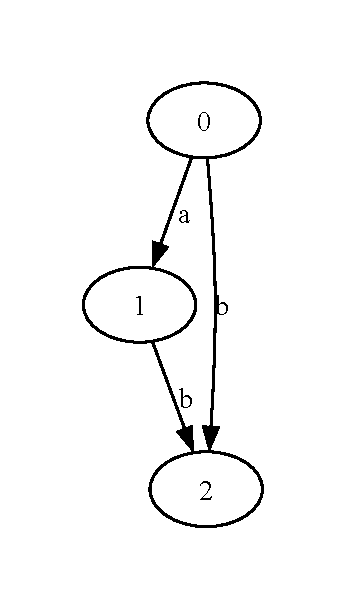
\includegraphics[width=0.5\linewidth]{testsuite/neg_demo} 
  \end{minipage}
  \hfill
% Right: verbatim DOT code
  \begin{minipage}{0.45\textwidth}
\begin{verbatim}
digraph neg_demo {
  0;
  1;
  2;
  0 -> 1 [label="a"];
  0 -> 2 [label="b"];
  1 -> 2 [label="b"];
}
\end{verbatim}
\end{minipage}  
\caption{An edge-labelled graph and its dot format specification}
\label{fig:neg_demo}
\end{figure}



\subsection{Edge Predicates}

At the heart of Greggle's regular expressions are \emph{edge-level
predicates}.  Intuitively, an edge predicate $P$ is a boolean
expression that can be evaluated on the label set $L$ of a single
edge, yielding true or false.  Greggle provides the following primitive
constructors:
\begin{itemize}[leftmargin=*]
  \item Atomic label test: \texttt{a} is true on an edge whose label
        set contains the symbol \texttt{a}.
  \item Wildcard: \texttt{dot} is true on every edge, regardless of
        its label set (analogous to ``.'' in traditional regular
        expressions).
  \item Source-node lift: \texttt{P@} is true on an edge when the
        string regular expression \texttt{P} matches the label of the
        source node of that edge.
  \item Sink-node lift: \texttt{@P} is true on an edge when the
        string regular expression \texttt{P} matches the label of the
        sink node of that edge.
  \item Negation: \texttt{(negate $P$)} is true when $P$ is false on
        that edge.
  \item All-of: \texttt{(all-of $P_1$ $P_2$ $\dots$)} is true when
        each $P_i$ is true on that edge.
  \item Some-of: \texttt{(some-of $P_1$ $P_2$ $\dots$)} is true when
        at least one $P_i$ is true on that edge.
\end{itemize}
These constructors can be nested arbitrarily.  As convenient
shorthand, a leading tilde on an atom is interpreted as negation, so
\texttt{\textasciitilde a} is equivalent to \texttt{(negate a)}.

For example:
\begin{itemize}[leftmargin=*]
  \item \texttt{a} holds on an edge with labels $\{\texttt{a},\texttt{b}\}$;
        \texttt{\textasciitilde a} does not.
  \item \texttt{(all-of a b)} holds on an edge with labels
        $\{\texttt{a},\texttt{b}\}$ but not on one with just
        $\{\texttt{a}\}$.
  \item \texttt{(some-of b c)} holds on an edge with labels
        $\{\texttt{b},\texttt{c}\}$ and also on one with labels
        $\{\texttt{b}\}$ or $\{\texttt{c}\}$.
  \item \texttt{MID@} holds on an edge whose source node label
        matches the regex \texttt{MID}.
  \item \texttt{@TARGET} holds on an edge whose sink node label
        matches the regex \texttt{TARGET}.
\end{itemize}

\subsection{Path Expressions}

Path expressions describe sets of finite paths in the graph.  They are
regular expressions whose atomic symbols are edge predicates.  The
syntax is:
\begin{itemize}[leftmargin=*]
  \item \texttt{P}, where $P$ is an edge predicate, denotes a single
        edge on which $P$ holds.
  \item \texttt{(concat $r_1$ $r_2$ $\dots$ $r_n$)} denotes
        concatenation: paths formed by following a subpath in $r_1$,
        then $r_2$, etc.
  \item \texttt{(alt $r_1$ $r_2$ $\dots$ $r_n$)} denotes alternation:
        a path is accepted if it is accepted by some $r_i$.
  \item \texttt{(star $r$)} denotes Kleene star, any finite
        concatenation of paths in the language of $r$ (including the
        empty path).
  \item \texttt{(plus $r$)} denotes one-or-more repetitions of $r$.
\end{itemize}

In practice, an atomic symbol \texttt{a} is treated as the edge
predicate testing for label \texttt{a}, and we omit the explicit
\texttt{sym} constructor sometimes found in other presentations.

\subsection{Query Expressions}

Building on path expressions, Greggle defines expressions that relate
node variables:
\begin{itemize}[leftmargin=*]
  \item \texttt{(exists-path x y $r$)} is true under an assignment of
        nodes to variables $x$ and $y$ when there exists a path from
        $x$ to $y$ in the graph whose sequence of edge labels is
        accepted by the path expression $r$.
  \item \texttt{(match x $p$)} is true when the label of node $x$
        (as taken from the DOT identifier or other node name) matches
        the string regular expression $p$ in the usual sense of
        \texttt{std::regex\_match}.
  \item \texttt{(no-edge x y)} is true when there is \emph{no} edge
        from $x$ to $y$ in the graph.
  \item \texttt{(no-connection x y)} is true when there is no edge
        between $x$ and $y$ in either direction (neither $x \to y$ nor
        $y \to x$).
  \item \texttt{(same x y)} is true when $x$ and $y$ are assigned the
        same node.
  \item \texttt{(different x y)} is true when $x$ and $y$ are assigned
        different nodes.
  \item \texttt{(and $e_1$ $e_2$ $\dots$ $e_n$)} is true when all
        subexpressions are true under the current assignment.
  \item \texttt{(or $e_1$ $e_2$ $\dots$ $e_n$)} is true when at least
        one $e_i$ is true.
  \item \texttt{(not $e$)} is the logical complement.
  \item \texttt{(exists (x y $\dots$) $e$)} existentially quantifies
        over the listed variables, projecting them out of the final
        result.
\end{itemize}

The free variables of an expression are those that are not bound by an
enclosing \texttt{exists}.  Evaluating a query on a fixed graph yields
a relation over the free variables; the query tool displays this as a
set of satisfying bindings.

\section{Informal Semantics}

\subsection{Path Semantics}

The semantics of path expressions follow the usual automata-theoretic
view of regular expressions.  For each regular expression $r$, we
construct a finite-state automaton that reads the labels along a path,
where each symbol corresponds to an edge predicate.  A path in the
graph is accepted by $r$ if the sequence of edge label sets along the
path causes the automaton to reach an accepting state.

Operationally, Greggle builds a nondeterministic finite automaton
(NFA) from the regular expression and performs a breadth-first search
over the product of graph nodes and NFA states.  An edge
$(u,L,v)$ can be taken for a particular NFA transition labelled by
predicate $P$ precisely when $P$ evaluates to true on $L$.
Whenever a product state $(u,q)$ is reached with $q$ accepting, the
pair $(x=u,y)$ is recorded as satisfying the corresponding
\texttt{exists-path} predicate.

\subsection{Relational Semantics}

The top-level semantics of queries is relational.  For a given query
$e$ with free variables $x_1,\dots,x_n$, evaluation on a graph $G$
produces a relation $R_e \subseteq V^n$:
\begin{itemize}[leftmargin=*]
  \item For \texttt{(exists-path x y $r$)}, $R_e$ is the set of pairs
        $(u,v)$ such that there is a path from $u$ to $v$ in $G$ whose
        label sequence is accepted by $r$.
  \item For \texttt{(match x $p$)}, $R_e$ is the set of singletons
        $(u)$ such that the node label associated with $u$ matches the
        string regular expression $p$.
  \item For \texttt{(no-edge x y)}, $R_e$ is the set of pairs $(u,v)$
        such that there is \emph{no} edge $(u,L,v) \in E$ for any
        label set $L$.
  \item For \texttt{(no-connection x y)}, $R_e$ is the set of pairs
        $(u,v)$ such that neither $(u,L,v)$ nor $(v,L',u)$ is in $E$
        for any label sets $L,L'$; that is, there is no edge between
        $u$ and $v$ in either direction.
  \item For \texttt{(same x y)}, $R_e$ is the set of pairs $(u,u)$
        (equality of the two variables over the node domain).
  \item For \texttt{(different x y)}, $R_e$ is the set of pairs
        $(u,v)$ with $u \neq v$ (inequality of the two variables).
  \item \texttt{(and $e_1$ $e_2$)} corresponds to relational
        intersection (natural join on shared variables).
  \item \texttt{(or $e_1$ $e_2$)} corresponds to relational union.
  \item \texttt{(not $e$)} corresponds to relational complement with
        respect to the full Cartesian product of the domains of the
        free variables.
  \item \texttt{(exists (x\_i) $e$)} corresponds to existential
        projection, eliminating the quantified variables from the
        result relation.
\end{itemize}

Internally, Greggle represents these relations symbolically using a
BDD-backed finite-domain layer, but the user-facing behaviour matches
the relational view sketched above.

\section{Examples}

\subsection{An Example Graph}

Figure~\ref{fig:handmade-sample} shows an example graph with mixed labels, illustrating the style of graphs
Greggle is designed to work with.  Nodes represent network states,
edges represent transitions labelled by actions or propositions.

\begin{figure}[t]
  \centering
  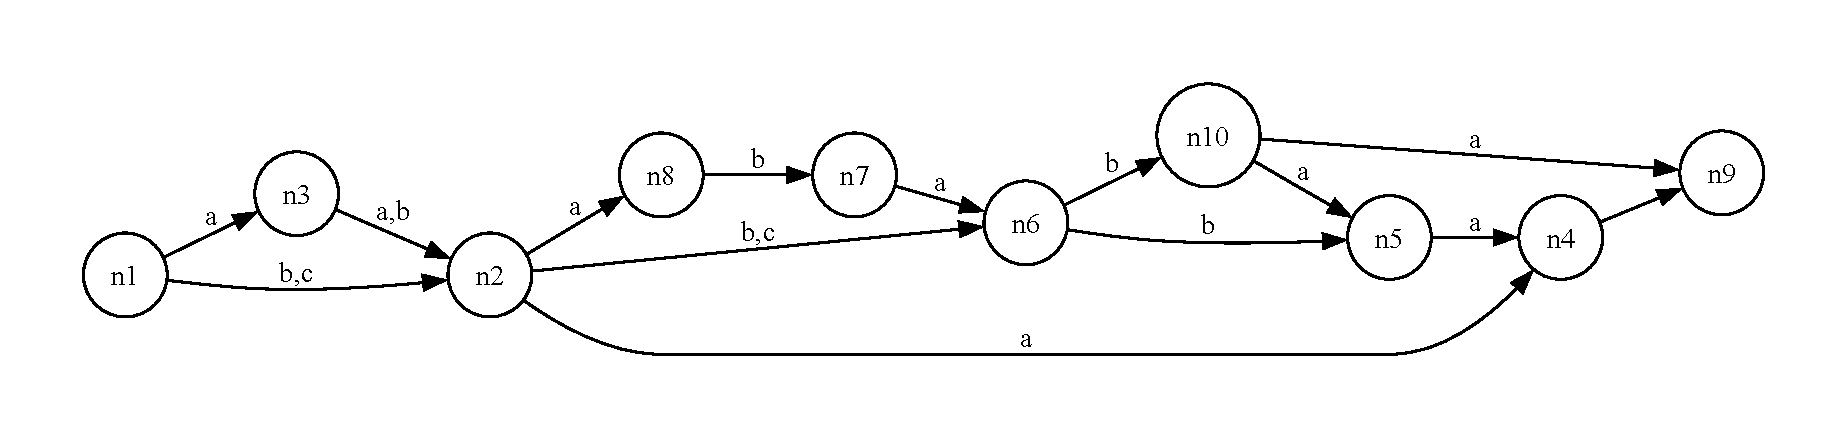
\includegraphics[width=\textwidth]{testsuite/handmade_sample.pdf}
  \caption{Example labelled graph used in several path queries.}
  \label{fig:handmade-sample}
\end{figure}

On this graph, one can express queries such as:
\begin{itemize}[leftmargin=*]
  \item Paths starting with \texttt{a} and then repeating
        \texttt{b\,a} one or more times:
        \begin{verbatim}
(exists-path x y (concat a (plus (concat b a))))
        \end{verbatim}
  \item Pairs of nodes connected by a path of only \texttt{c}-edges
        and also by a path matching the previous pattern:
        \begin{verbatim}
(and (exists-path x y (star c))
     (exists-path x y (concat a (plus (concat b a)))))
        \end{verbatim}
\end{itemize}
These examples exercise nested regular expressions and relational
conjunction, and correspond closely to the more detailed examples used
in the original experiments.

\subsection{Negated Edge Predicate}

Consider again the small graph \texttt{neg\_demo} mentioned in section \ref{sectionOnGraphs}.
The query
\begin{verbatim}
(exists-path x y ~a)
\end{verbatim}
asks for all pairs $(x,y)$ such that there exists a single edge from
$x$ to $y$ whose label set does \emph{not} contain \texttt{a}.  On
this graph, the satisfying bindings are:
\begin{verbatim}
Satisfying bindings:
x=0 y=2
x=1 y=2
\end{verbatim}
corresponding exactly to the two edges labelled \texttt{b}.

\subsection{All-of and Some-of}

Now consider the graph in Figure \ref{fig:all_some_demo}.
\begin{figure}[h]
  \centering
  % Left: verbatim DOT code
  \begin{minipage}{0.45\textwidth}
\begin{verbatim}
digraph all_some_demo {
  0;
  1;
  2;
  0 -> 1 [label="a,b"];
  0 -> 2 [label="a"];
  1 -> 2 [label="b,c"];
}
\end{verbatim}
  \end{minipage}\hfill
  % Right: diagram image
  \begin{minipage}{0.45\textwidth}
    \centering
    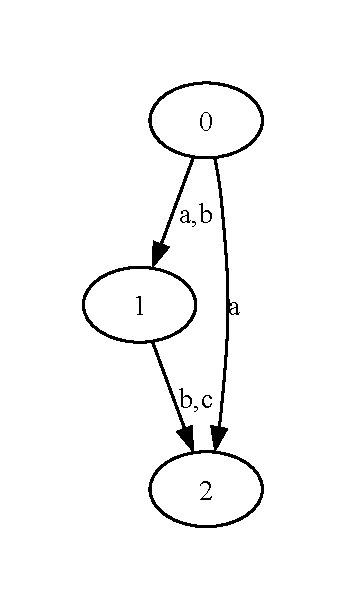
\includegraphics[width=0.5\linewidth]{testsuite/all_some_demo} 
  \end{minipage}
  \caption{A graph with multi-labelled edges}
    \label{fig:all_some_demo}
\end{figure}


The query
\begin{verbatim}
(exists-path x y (all-of a b))
\end{verbatim}
asks for all edges that have \emph{both} labels \texttt{a} and
\texttt{b}.  On this graph, the only such edge is $0 \to 1$, and the
result is:
\begin{verbatim}
Satisfying bindings:
x=0 y=1
\end{verbatim}

The query
\begin{verbatim}
(exists-path x y (some-of b c))
\end{verbatim}
asks for all edges that have \texttt{b} or \texttt{c} (or both).  Here
both $0\to 1$ and $1\to 2$ satisfy this predicate, yielding:
\begin{verbatim}
Satisfying bindings:
x=0 y=1
x=1 y=2
\end{verbatim}

These examples demonstrate how edge-level predicates can succinctly
express conditions involving the presence or absence of multiple
labels on a single edge.

\subsection{Wildcard and Relational Predicates}

The \texttt{dot} predicate acts as a wildcard edge test: it is true on
every edge, regardless of its label set.  On the graph
\texttt{neg\_demo} from Section~\ref{sectionOnGraphs}, the query
\begin{verbatim}
(exists-path x y dot)
\end{verbatim}
asks for all single-edge connections in the graph, and yields exactly
the set of edges:
\begin{verbatim}
Satisfying bindings:
x=0 y=1
x=0 y=2
x=1 y=2
\end{verbatim}

The predicate \texttt{(no-edge x y)} expresses the absence of a
directed edge from $x$ to $y$, while \texttt{(no-connection x y)}
expresses the absence of any edge between $x$ and $y$ in either
direction.  On \texttt{neg\_demo}, for example, \texttt{(no-connection
  x y)} holds only when $x$ and $y$ are the same node, since every
unordered pair of distinct nodes is joined by at least one edge.

Finally, the predicates \texttt{(same x y)} and \texttt{(different x
  y)} implement equality and inequality over node variables.  On a
graph with nodes $0,1,2$, \texttt{(same x y)} yields bindings
\texttt{x=0,y=0}, \texttt{x=1,y=1}, \texttt{x=2,y=2}, while
\texttt{(different x y)} yields all pairs where the node components
are distinct.  These relational primitives make it easy to combine
path-based conditions with simple structural constraints on node
assignments.

Node-label tests can also be lifted into edge predicates inside a path
expression.  If \texttt{P} is a string regular expression over node
labels, then \texttt{P@} tests the source node of the edge and
\texttt{@P} tests the sink node.  For instance,
\begin{verbatim}
(exists-path x y (all-of a @TARGET))
\end{verbatim}
matches \texttt{a}-labelled edges whose sink node label matches
\texttt{TARGET}, while
\begin{verbatim}
(exists-path x y (all-of a MID@))
\end{verbatim}
matches \texttt{a}-labelled edges whose source node label matches
\texttt{MID}.  Since these are ordinary edge predicates, they compose
normally with \texttt{negate}, \texttt{all-of}, and \texttt{some-of}.

As a final illustration, consider a graph whose node labels are
strings such as \texttt{A}, \texttt{AB}, \texttt{B1}, \texttt{Z},
with edges labelled by atomic propositions \texttt{a}, \texttt{b}.
The query
\begin{verbatim}
(and (match x "A.*")
     (exists-path x y a))
\end{verbatim}
asks for all pairs $(x,y)$ such that the label of $x$ matches the
pattern \texttt{A.*} and there is an edge labelled \texttt{a} from
$x$ to $y$.  On a graph where there is an \texttt{a}-edge from
\texttt{A} to \texttt{Z} but only a \texttt{b}-edge from \texttt{AB}
to \texttt{Z}, the only satisfying binding is
\texttt{x=A,y=Z}, combining a label-based filter with a path
predicate.

\section{DOT-Based Query Tool}

The Greggle query tool is a command-line program that takes a DOT file
and a query expression as arguments, and prints the satisfying
bindings.  Its usage is:
\begin{verbatim}
greggle <graph.dot> "<query in lisp syntax>"
\end{verbatim}
where the query must be quoted so that it is passed as a single
argument.

Internally, the tool:
\begin{enumerate}[leftmargin=*]
  \item Parses the DOT file, assigning each node identifier a unique
        integer index and collecting edge label sets.
  \item Parses the query S-expression, building the abstract syntax
        tree for path and edge predicates.
  \item Evaluates the query on the graph to obtain a relation over the
        free variables.
  \item Prints each satisfying binding as a line of the form
        \texttt{x=nodeLabel y=nodeLabel}, mapping internal node
        indices back to the original DOT labels.
\end{enumerate}

For example, running the tool on \texttt{neg\_demo.dot} with the
negated edge predicate query produces:
\begin{verbatim}
Satisfying bindings:
x=0 y=2
x=1 y=2
\end{verbatim}
matching the hand analysis above.

\section{Conclusion}

Greggle offers a compact and expressive language for regular path
queries over DOT-described graphs.  By combining regular expressions
with edge-level boolean predicates and relational operators, it
supports a range of natural graph queries, including those that depend
on the presence or absence of specific labels on individual edges.

Although the underlying implementation uses BDDs and symbolic
representations of relations, users interact only with graphs in DOT
format and queries in a small S-expression language.  The examples
presented here illustrate both the core regular path constructs and
the newer edge predicate primitives, which together provide a flexible
basis for experimenting with graph queries in a concise setting.

\section{Future Work}

The current system supports negation at the relational level (via
\texttt{(not $e$)} on expressions) and at the edge level (via
\texttt{(negate $P$)} and the \texttt{\textasciitilde a} shorthand on predicates),
but does not provide a general \emph{regex-level} negation operator
inside path expressions themselves.  One natural idea is to allow
expressions such as
\begin{verbatim}
(exists-path x y (negate-regexp r))
\end{verbatim}
where \texttt{(negate-regexp r)} would match exactly those paths whose
label sequences are \emph{not} in the language denoted by $r$.

Language-theoretically, this corresponds to complementing the regular
language defined by $r$.  In an automata-based setting this is usually
achieved by first determinizing the NFA for $r$ to a complete DFA
over a chosen alphabet, and then flipping accepting and
non-accepting states.  In the current implementation, however, path
expressions are compiled only to NFAs and evaluated by a breadth-first
search over product states $(\text{graph node},\text{NFA state})$.
There is no DFA construction or automaton-level complement.

Moreover, as soon as one wants regex-level negation as a
subexpression, for example inside concatenation or repetition, one
must be precise about the ambient alphabet (all labels in the graph,
all labels appearing anywhere in the regexes, etc.) and ensure that
the resulting construction behaves compositionally.  This suggests
that supporting a general \texttt{negate-regexp} operator would
require:
\begin{itemize}[leftmargin=*]
  \item Extending the regex syntax with an explicit negation form.
  \item Building DFAs (at least conceptually) for subexpressions, with
        a clear choice of alphabet and completion strategy.
  \item Implementing language complement at the automaton level, and
        then integrating the resulting automata into the existing
        path-evaluation BFS.
\end{itemize}
While conceptually straightforward, this is not a small local change
and has been left for future work.  For many practical cases, the
combination of relational negation on whole path predicates and
edge-level predicates already provides substantial expressive power,
but exploring full regex-level negation remains an interesting
extension.  For example, the expression
\begin{verbatim}
(not (exists-path x y (negate-regexp R)))
\end{verbatim}
would have the natural semantics that \emph{every} path from $x$ to
$y$ satisfies $R$, which would be a welcome addition to the
expressive power of the language.

\appendix
\section*{Appendix: Implementation Overview}

This appendix sketches how Greggle is implemented, focusing on data
structures and algorithms rather than concrete code.

\subsection*{Overall Architecture}

At a high level, evaluation proceeds in three stages:
\begin{enumerate}[leftmargin=*]
  \item \textbf{Parsing:} The input graph (e.g.\ a DOT file) is parsed
        into an internal labelled graph representation.  The query
        S-expression is parsed into an abstract syntax tree (AST)
        whose nodes represent expressions (\texttt{exists-path},
        \texttt{and}, \texttt{or}, \texttt{not}, \texttt{exists}) and
        path expressions (regular expressions built from edge
        predicates).
  \item \textbf{Path evaluation:} For each \texttt{exists-path}
        subexpression, a nondeterministic finite automaton (NFA) is
        constructed from the regular expression, and a search is
        performed over the product of graph nodes and NFA states to
        compute a binary relation over node variables.
  \item \textbf{Relational composition:} The relations produced by
        \texttt{exists-path} are combined using relational operators
        (intersection, union, projection, complement), implemented
        symbolically using BDD-backed finite-domain relations.
\end{enumerate}

\subsection*{Path Evaluation via NFA}

Each path expression is compiled into a small NFA.  States are
classified as accepting or non-accepting, and transitions are labelled
either by edge predicates (for consuming one edge) or by
epsilon-transitions (for moving between states without consuming an
edge).  Regular expression constructs are handled in the standard
way:
\begin{itemize}[leftmargin=*]
  \item A symbol (edge predicate) becomes a two-state NFA with a single
        consuming transition.
  \item Concatenation connects the end states of each component
        using epsilon-transitions.
  \item Alternation introduces a fresh start and end state and connects
        them via epsilon-transitions to and from each component.
  \item Star and plus introduce loops via epsilon-transitions to allow
        repeated traversal.
\end{itemize}

To evaluate \texttt{(exists-path x y $r$)} on a graph $G$, the system
runs a breadth-first search over pairs $(u,q)$ where $u$ is a graph
node and $q$ is an NFA state.  For each start node $s$, the search is
initialized at all NFA states reachable from the NFA start by
epsilon-transitions, paired with $s$.  The algorithm repeatedly:
\begin{itemize}[leftmargin=*]
  \item Dequeues a pair $(u,q)$.
  \item If $q$ is accepting, records $(x=u,y=u')$ as satisfying, where
        $u'$ is the current node in that pair.
  \item For each outgoing edge $(u,L,v)$ in $G$ and each NFA transition
        from $q$ labelled by edge predicate $P$, checks whether $P$
        holds on the label set $L$.  If so, it follows that transition
        to a new NFA state $q'$, computes the epsilon-closure of $q'$,
        and enqueues any new pairs $(v,q'')$ not seen before.
\end{itemize}

The result of this search is a set of node pairs $(s,t)$ that
constitute the relation for \texttt{exists-path} over the variables
$(x,y)$.

\subsection*{Symbolic Relations with BDDs}

Relations over node variables are represented symbolically using a
finite-domain BDD layer.  Each logical variable is associated with a
finite-domain identifier; the underlying BDD package provides
operations to represent and manipulate finite-domain predicates
over these identifiers.  A relation is thus encoded as a BDD whose
variables correspond to the finite-domain variables for the logical
variables.

Given a tuple of node values $(v_1,\dots,v_k)$ over variables
$(x_1,\dots,x_k)$, the system constructs a conjunction of
finite-domain predicates stating that each variable $x_i$ equals
value $v_i$, and ORs these into the BDD representing the relation.
From this representation, the following relational operations are
implemented:
\begin{itemize}[leftmargin=*]
  \item \textbf{Union} and \textbf{Intersection} via BDD disjunction
        and conjunction, respectively.
  \item \textbf{Set difference} by conjunction with the negation of
        the other relation.
  \item \textbf{Projection} by existential quantification over the
        finite-domain variables corresponding to quantified logical
        variables.
  \item \textbf{Complement} by BDD negation, with respect to the full
        product domain of the participating variables.
\end{itemize}

\subsection*{Edge Predicate Evaluation}

Edge predicates are represented as small trees with nodes for atomic
tests and boolean connectives (negation, all-of, some-of).  Each
atomic test stores a label name.  Evaluation of a predicate $P$ on an
edge is implemented by recursively traversing this tree:
\begin{itemize}[leftmargin=*]
  \item An atomic predicate compares its label name to the edge's label
        set.
  \item A negation node inverts the result of its child.
  \item An all-of node checks that all child predicates hold.
  \item A some-of node checks that at least one child predicate holds.
\end{itemize}

During NFA traversal, these predicates are used to decide which
transitions are enabled on a given edge.  This design cleanly
separates path structure (handled by the NFA) from local label
conditions (handled by predicate evaluation).

\subsection*{Query Tool Pipeline}

The command-line query tool ties these pieces together:
\begin{enumerate}[leftmargin=*]
  \item Parses a DOT snippet or other graph description into the
        internal graph structure.
  \item Parses the query S-expression into the expression and path
        ASTs, including edge predicates.
  \item Evaluates the expression on the graph, constructing and
        combining symbolic relations as needed.
  \item Traverses the resulting relation and prints each satisfying
        binding, mapping internal node indices back to external node
        identifiers where appropriate.
\end{enumerate}

This architecture allows Greggle to support expressive regular path
queries with edge-level predicates while keeping the implementation
modular: path processing is localized to the NFA construction and
product search, whereas relational composition and quantification are
handled uniformly by the BDD-backed finite-domain layer.

\bibliographystyle{plain}
\bibliography{references}
\end{document}

